%% ICTC 2026 — IWETRIAI : 한글판 (검토용, XeLaTeX로 컴파일)
%% 영어 제출본 main.tex와 동일 구조. 컴파일: xelatex main_kr.tex (TinyTeX)
\documentclass[conference]{IEEEtran}
\IEEEoverridecommandlockouts
\usepackage{fontspec}
\setmainfont{Malgun Gothic}
\usepackage{amsmath,amssymb,amsfonts}
\usepackage{graphicx}
\usepackage{booktabs}
\usepackage{xcolor}

\begin{document}

\title{검증의 신뢰성이 병목이다, 모델 용량이 아니라:\\
소비자 라이프로그 센서로부터 수면지표를 예측하는\\
시간이동-인지 다중소스 앙상블}

\author{
\IEEEauthorblockN{서동현 (Donghyun Seo)}
\IEEEauthorblockA{\textit{Independent Researcher}\\
Republic of Korea \\
tjehdgus113@gmail.com}
}

\maketitle

\begin{abstract}
스마트폰·스마트워치 센서의 전날 하루 기록으로 그날 밤 수면에 대한 7개의 이진(0/1) 지표를 예측하는
문제를 다룬다(ETRI 2026 휴먼이해 AI 챌린지). 이 과제는 실제 라이프로그 환경에서 흔하지만 함께 다뤄진
적이 드문 두 가지 어려움을 동시에 안고 있다: 매우 작은 표본(피험자 10명, 학습 450박)과 \emph{시간적
분포 이동}(평가 대상 밤들이 학습 밤들보다 시간상 뒤쪽에 몰림)이다. 우리는 그래디언트 부스팅 트리,
시퀀스 신경망, 동결된 비전 파운데이션 모델, 액티그래피식 수면 재구성, 라벨 자기상관 이웃 모델을 아우르는
9개 소스 앙상블을 구축하고 타겟별 greedy 블렌딩으로 결합한다. 우리의 핵심 발견은 방법론적이다:
시간이동과 작은 표본 하에서 진짜 병목은 모델 용량이 아니라 \emph{검증의 신뢰성}이다. 무작위 $k$-겹
교차검증은 일반화되지 않는 변화를 체계적으로 보상하는 반면, 실제로 held-out 데이터에 전이되는 개선은
두 종류뿐이다 — 다중 시드 분산 감소와 \emph{forward-chaining(시간이동 인지) 재가중}. 우리 최종 제출물은
Average Log-Loss $0.578$을 기록하며, 더 중요하게는 통제된 ablation이 일반화된 개선을 만든 것은 모델 용량
추가가 아니라 규율 있는 시간이동-인지 검증임을 보인다. 또한 그 결과로 나타난 데이터 천장이 구조적임을
정직하게 분석한다: 7개 라벨 중 4개는 입력에 없는 임상용 수면측정기에서 파생되기 때문이다.
\end{abstract}

\begin{IEEEkeywords}
라이프로그, 수면 예측, 앙상블 학습, 분포 이동, 시계열 교차검증, 소표본 학습
\end{IEEEkeywords}

\section{서론}
소비자 웨어러블·스마트폰은 풍부한 행동·생리 신호를 수동적으로 기록하므로, 전용 임상장비 없이도 일상
기기로 수면질을 추론할 가능성을 연다. ETRI 2026 휴먼이해 AI 챌린지는 그런 과제를 정형화한다: 12종
센서의 하루치 기록으로 \emph{그날 밤} 수면의 7개 이진 지표를 예측. 세 지표(Q1--Q3)는 설문 결과(수면질,
피로, 스트레스)로 \emph{각 개인의 장기 평균 대비}로 이진화된다. 나머지 넷(S1--S4)은 미국수면재단(NSF)
가이드라인 — 총수면시간, 수면효율, 입면지연, 중도각성 — 의 충족 여부를 인코딩한다~\cite{nsf}.

두 가지 성질이 이 과제를 유난히 까다롭게 만든다. 첫째, 데이터가 \emph{작다}: 피험자 10명에서 나온 학습
450박과 같은 사람들의 평가 250박. 둘째, \emph{시간이동}이 있다: 평가 밤들이 각 피험자의 학습 구간보다
대체로 뒤에 있다(그림~\ref{fig:shift}). 이 둘이 합쳐지면 모델이 피험자별 특이패턴을 외우기 쉽고, 더
위험하게는 밤을 \emph{무작위로 섞어} 계산한 검증 점수가 실제 평가셋 대비 \emph{낙관적으로 편향}된다.

채점지표는 macro(라벨 평균) 로그 로스(식~\ref{eq:logloss})로, 잘 보정된 확률을 보상하고 자신 있는 오답을
크게 벌한다(낮을수록 좋음).
\begin{equation}
\mathcal{L} = \frac{1}{7}\sum_{j=1}^{7}
-\frac{1}{N}\sum_{i=1}^{N}\Big[y_{ij}\log \hat p_{ij}+(1-y_{ij})\log(1-\hat p_{ij})\Big].
\label{eq:logloss}
\end{equation}

\textbf{기여 3가지:}
\begin{itemize}
\item 소비자 센서 수면지표 예측을 위한 9개 다중소스 앙상블 — NSF 라벨을 직접 겨냥하는 액티그래피식 수면
재구성과, 센서 시계열에 직교적 시각을 주입하는 동결 비전모델 임베딩 포함(제~\ref{sec:method}절).
\item 논문의 중심 주장으로 삼는 경험적 관찰: 시간이동·소표본 하에서 작동하는 병목은 검증의 신뢰성이다.
무작위 교차검증은 속이고, 분산 감소와 forward-chaining 재가중만 held-out에 전이된다
(제~\ref{sec:exp}--\ref{sec:disc}절).
\item 이 과제의 달성 가능 성능을 제한하는 구조적 데이터 천장의 정직한 규명 — 입력에 없는 임상 모달리티에
뿌리(제~\ref{sec:disc}절).
\end{itemize}

\section{데이터와 문제 설정}
\label{sec:data}
각 밤은 \texttt{lifelog\_date}(센서가 관측된 전날)와 \texttt{sleep\_date}에 연결된다. 12개 센서 계열:
워치의 심박·보행계, 폰의 화면·충전·활동상태·주변소리·GPS·조도·Wi-Fi·BLE·앱사용. 샘플링·커버리지가 크게
다르며, 특히 워치 심박은 타임스탬프마다 초단위 배열을 저장하고 밤에 가장 희박하다.

\textbf{라벨 구조.} 두 라벨 계열은 서로 다른 귀납 편향을 요구한다. Q1--Q3은 개인 평균 대비라서 피험자마다
양성률 편차가 크고(라벨·피험자에 따라 약 0.15--0.85), 이는 \emph{피험자내 정규화}와 Q 타겟의 순위 기반
처리를 동기화한다. 반면 S1--S4는 절대 임상 임계라서 피험자별 충족률이 비교적 안정적이고, 개인 기저율
prior가 강한 앵커가 된다.

\textbf{미관측 모달리티.} 결정적으로, S1--S4는 12개 입력에 \emph{없는} Withings 수면측정기(머리맡 기기)로
계산된다. 폰·워치는 그 라벨이 임계 처리하는 양(총수면시간·효율·지연·각성)을 \emph{간접 추정}할 수 있을
뿐이다. 이 격차가 우리가 보고하는 구조적 천장의 원천이다.

\textbf{시간이동.} 그림~\ref{fig:shift}은 학습·평가 밤의 \texttt{sleep\_date}를 피험자별로 그린다. 모든
피험자에서 평가 밤(주황)이 학습 밤(초록)보다 뒤로 뻗는다. 밤을 균일하게 섞는 검증은 배포 모델이 결코
보지 못할 분포에서 평가하는 셈이다.

\begin{figure}[t]
\centering
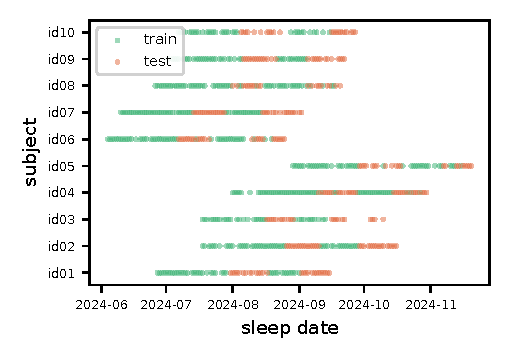
\includegraphics[width=\columnwidth]{figs/shift.pdf}
\caption{피험자별 학습(초록)·평가(주황) 밤의 시간 분포. 평가 밤이 일관되게 뒤에 있어 모델이 견뎌야 할
분포 이동을 정의한다. 이 관찰 하나가 제~\ref{sec:method}절의 forward-chaining 검증을 동기화한다.}
\label{fig:shift}
\end{figure}

\section{방법}
\label{sec:method}
3단 구조를 따른다: (i) 다양한 베이스 소스 구축, (ii) 타겟별 greedy 블렌딩, (iii) 시간·정의 인지 보정.
모든 피처는 피험자내 정규화해 "그 사람 습관 대비 오늘"을 인코딩하며, 이는 Q 라벨의 상대적 정의와
일치한다.

\subsection{피처 엔지니어링}
각 센서를 (피험자, \texttt{lifelog\_date}) 단위로 시간대 윈도우(낮/저녁/취침전/밤/아침 등)별 통계로
집계하고, 야간 윈도우는 올바른 달력 밤에 귀속한다. 그 위에 피험자내 시계열 파생(lag 차분·이동평균·지수평균·누적평균)으로
개인 기준선을 인코딩한다. 심박 배열은 생리적으로 불가능한 값을 제거한 뒤 분단위 평균/최소/최대/표준편차로
축약한다.

\subsection{베이스 소스}
메커니즘 다양성을 기준으로 9개 소스를 구성한다:
\begin{enumerate}
\item \textbf{트리.} LightGBM~\cite{lightgbm} + CatBoost~\cite{catboost} + ExtraTrees 가중평균.
ExtraTrees 중요도로 상위 150피처를 선택하고, pseudo-labeling(확신 임계 $0.85$)으로 확신 높은 평가행을
학습에 추가한다.
\item \textbf{Prior.} 피험자 과거 라벨 평균 — 특히 절대 S 라벨에서 강한 앵커.
\item \textbf{시퀀스망(GRU·BiLSTM·TCN~\cite{tcn}·Attention).} 각각 1D-CNN 인코더 + 시퀀스 모듈 + 피험자
임베딩 + 7헤드. 각 구조를 8개 random seed로 학습해 평균(DLens)한다. N=450에서 신경망은 고분산이라 시드
평균이 분산을 줄인다(가중치 평균과 같은 발상)~\cite{swa}.
\item \textbf{비전 임베딩(SigLIP-Large).} 센서를 2D 이미지로 만들어 \emph{동결} SigLIP-Large 비전
트랜스포머~\cite{siglip}에 통과, 풀링 임베딩을 부스팅에 투입한다. 가중치는 학습하지 않으며, 트리·시퀀스와
직교하는 일반 시각 인코딩을 제공한다.
\item \textbf{수면 재구성(SleepTree2).} 야간 움직임·심박·충전으로 주수면 구간을 재구성해 분단위 총수면/효율/지연/각성
추정과 NSF 임계 플래그를 만들어 트리에 투입한다 — S1--S4 직격.
\item \textbf{이웃(Neighbor).} 같은 피험자의 \emph{다른} 밤 라벨을 날짜 지수가중 평균(leave-one-out)한다.
수면 결과의 날짜 자기상관을 활용한다.
\end{enumerate}
추가로 700일 전체를 30분 bin 행동으로 transductive 비음수 행렬분해~\cite{nmf}한 라벨-free
\emph{daystate} 표현을 만들어 Q1/Q2 예측 라우팅에 사용한다.

\subsection{블렌딩}
타겟마다 prior 앵커에서 출발해 $\pm 0.05/0.10$ 스텝 greedy coordinate descent로 식~(\ref{eq:logloss})를
최소화하는 소스 가중치를 선택한다. 그림~\ref{fig:srcll}처럼 어떤 단일 소스도 모든 라벨을 지배하지 못한다(수면
재구성이 여러 S에 최강, 이웃 모델이 한 Q에 최강) — 이것이 블렌딩이 이득을 보는 조건이다.

\subsection{정의·시간이동 인지 보정}
두 보정은 올바른 귀납 편향이 raw 용량보다 중요하다는 논문의 명제를 구현한다.

\textbf{Q 순위학습(pairwise).} Q 라벨이 개인 평균 대비이므로, 같은 피험자의 (양성 밤, 음성 밤) 쌍의 피처
차로 ridge logistic 모델을 적합하고~\cite{ranknet}, 그 결과를 logit 공간에서 스케일 잔차($\alpha{=}0.15$)로
Q1/Q2에 가산한다.

\textbf{S forward-chaining 재가중(핵심 레버).} 위 블렌드 가중치는 무작위 폴드에서 골랐는데, 이는
그림~\ref{fig:shift}이 경고하듯 시간이동된 평가셋을 반영하지 못한다. 그래서 S1/S4 가중치를
\emph{forward-chaining} 폴드로 다시 선택한다 — 앞쪽 $0.5$\,--\,$0.8$의 밤을 학습으로 쓰고 각 폴드가 다음
$20\%$ 블록을 검증하며 분할을 앞으로 미끄러뜨린다~\cite{bergmeir}. 그림~\ref{fig:forward}은 forward 방식이
in-sample에서만 좋아 보이는 소스에서 시간이동에 강건한 소스로 가중치를 옮김을 보인다. 이는 held-out에
전이된 단 두 변화 중 하나다.

\begin{figure}[t]
\centering
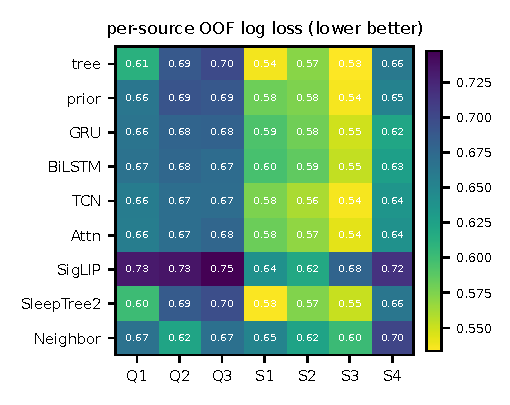
\includegraphics[width=\columnwidth]{figs/srcll.pdf}
\caption{소스별 라벨 OOF 로그 로스(밝을수록 좋음). 단일 소스가 모든 타겟을 지배하지 못해 타겟별 블렌드를
정당화한다.}
\label{fig:srcll}
\end{figure}

\begin{figure*}[t]
\centering
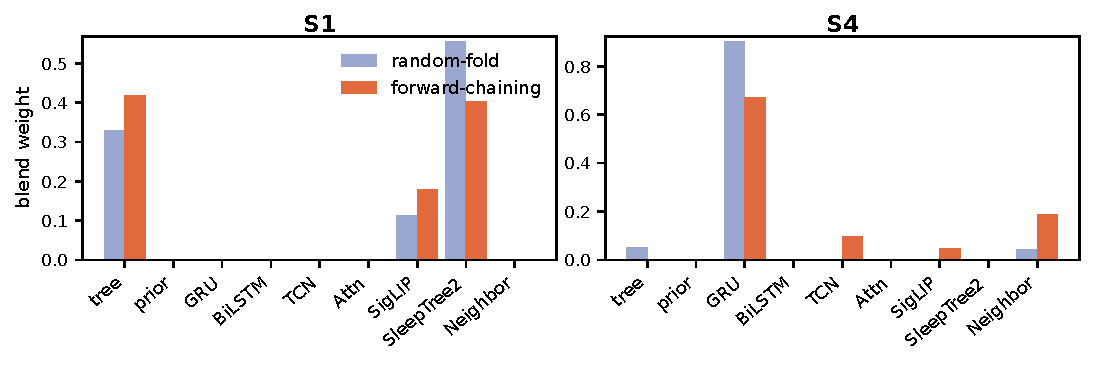
\includegraphics[width=0.92\textwidth]{figs/forward.pdf}
\caption{같은 9개 소스에 대해 무작위폴드(파랑)와 forward-chaining(주황) 검증으로 고른 S1·S4 블렌드
가중치. 시간이동-인지 방식이 시간상 앞으로 일반화되는 소스로 가중치를 재분배한다(예: S4에서 in-sample이
선호한 GRU에서 TCN·이웃 모델로). 이 재가중이 held-out 개선의 가장 큰 단일 원천이다.}
\label{fig:forward}
\end{figure*}

\section{실험}
\label{sec:exp}
macro 로그 로스(식~\ref{eq:logloss})를 보고한다(낮을수록 좋음, 무작위 추측은 $0.693$). 개발 중에는 내부
out-of-fold(OOF) 교차검증을, 최종 평가에는 챌린지 held-out 테스트 리더보드를 사용한다. 9소스 백본은
내부 OOF $0.584$, 정의·시간이동 보정을 더하면 최종 held-out \emph{Average Log-Loss $0.578$}에 도달한다.
절대 점수는 이 특정 벤치마크에 대해서만 의미가 있으므로, 분석은 무엇이 실제로 일반화되는지 훨씬 잘
말해주는 \emph{상대 비교}에 집중한다.

\textbf{전이된 것.} 표~\ref{tab:transfer}은 held-out 점수를 움직인 두 개선과 대표적 "환상" 변화를 대비한다.
다중 시드 DLens 평균은 작지만 신뢰성 있는 이득을 준다. S1/S4 forward-chaining 재가중이 최대 단일 레버로,
영향력을 강화할수록 held-out 성능이 단조 개선됐다. 반면 현재 최고 예측에서 크게 벗어난 후보들은 무작위폴드
OOF가 좋아져도 held-out을 \emph{악화}시켰고, 이 패턴은 시도한 약 20개 아이디어에서 반복됐다.

\begin{table}[t]
\caption{held-out에 전이되는 개선은 분산을 줄이거나 시간이동을 존중하는 것뿐이다. 무작위폴드 추정만
좋아진 변화는 전이되지 않는다.}
\label{tab:transfer}
\centering
\small
\begin{tabular}{@{}lcc@{}}
\toprule
변화 & 무작위폴드 OOF & held-out \\
\midrule
다중 시드 평균(DLens)        & 개선 & 개선(소폭) \\
forward-chaining S1/S4 재가중 & --   & \textbf{개선(최대)} \\
고-divergence ``새 신호'' 수정 & 개선 & 악화 \\
\bottomrule
\end{tabular}
\end{table}

\textbf{소스 다양성.} 블렌드가 통하는 이유는 다양성이다. 4개 시퀀스망은 예상대로 서로 상관이 높지만(최대
$0.98$), 메커니즘이 다른 계열들 — 트리·수면재구성·이웃·동결 비전 — 은 예측 상관이 $0.24$까지 낮다.
타겟별 블렌드가 활용하는 것은 계열 내 중복이 아니라 이 \emph{계열 간} 불일치이며, 그래서 각 소스가
단독으로는 약해도 블렌드가 모든 소스를 능가한다.

\section{논의}
\label{sec:disc}

\textbf{왜 무작위 CV가 여기서 속이나.} 작은 $N$, 피험자 10명, 시간상 앞으로의 평가셋이 결합되면 무작위
폴드는 두 방향으로 정보를 누설한다 — 같은 피험자의 인접 밤이 강하게 자기상관이고, 폴드가 테스트 때의 시간
간극을 재현하지 못한다. 결과적으로 무작위폴드 추정은 미묘한 과적합을 보상한다. forward-chaining 검증은 두
번째 누설을 제거하고 held-out 거동을 훨씬 잘 추적한다 — 우리 이득을 만든 것은 새 피처가 아니라 이 규율이다.

\textbf{구조적 천장.} 비전 모델, 여러 수면 재구성 변형, 심박변이 텍스처, 피험자별 모델, 외부 날씨·연결성
피처, 여러 라벨구조 exploit 등 광범위한 탐색에도 — 누수 없이 검증하면 어떤 "큰 베팅"도 held-out 이득을
내지 못했다. 이유는 구조적이다: S1--S4는 입력에 없는 임상 기기가 측정한 양을 임계 처리하고, Q2--Q3은
행동으로 느슨하게만 결정되는 주관 상태다. 폰·워치는 이를 일정 한계까지만 대리하며, 그것이 달성 가능 점수를
제한한다. 우리는 이 천장의 정직한 구획을 라이프로그 커뮤니티에 유용한 negative result로 본다.

\section{결론}
\label{sec:conc}
소표본·시간이동 하의 소비자 라이프로그 수면지표 예측에서, 결정적 요인은 모델 용량이 아니라 검증 프로토콜의
신뢰성이었다. 메커니즘이 다양한 9소스 앙상블이 강한 백본을 제공했지만, 실제로 일반화된 개선은 분산을
줄이거나(시드 평균) 시간이동을 존중하는(forward-chaining 재가중) 것들뿐이었다. 무작위폴드 추정만 좋아진
변화는 전이되지 않았다. 또한 미관측 임상 모달리티에 뿌리박은 구조적 데이터 천장을 기록했다. 이 관찰이
비슷하게 작고 이동된 라이프로그 데이터를 다루는 실무자들이 용량 추가보다 정직한 검증을 우선하도록 돕기를
바란다.

\section*{감사의 글}
ETRI 2026 휴먼이해 AI 챌린지 주최 측의 데이터셋과 평가 인프라에 감사드린다.

\begin{thebibliography}{00}
\bibitem{nsf} M. Hirshkowitz \emph{et al.}, ``National Sleep Foundation's sleep time
duration recommendations: methodology and results summary,'' \emph{Sleep Health},
vol.~1, no.~1, pp.~40--43, 2015.
\bibitem{lightgbm} G. Ke \emph{et al.}, ``LightGBM: A highly efficient gradient
boosting decision tree,'' in \emph{NeurIPS}, 2017.
\bibitem{catboost} L. Prokhorenkova \emph{et al.}, ``CatBoost: unbiased boosting with
categorical features,'' in \emph{NeurIPS}, 2018.
\bibitem{tcn} S. Bai, J. Z. Kolter, and V. Koltun, ``An empirical evaluation of
generic convolutional and recurrent networks for sequence modeling,''
\emph{arXiv:1803.01271}, 2018.
\bibitem{swa} P. Izmailov \emph{et al.}, ``Averaging weights leads to wider optima and
better generalization,'' in \emph{UAI}, 2018.
\bibitem{siglip} X. Zhai, B. Mustafa, A. Kolesnikov, and L. Beyer, ``Sigmoid loss for
language image pre-training,'' in \emph{ICCV}, 2023.
\bibitem{ranknet} C. Burges \emph{et al.}, ``Learning to rank using gradient
descent,'' in \emph{ICML}, 2005.
\bibitem{bergmeir} C. Bergmeir and J. M. Ben\'itez, ``On the use of cross-validation
for time series predictor evaluation,'' \emph{Information Sciences}, vol.~191,
pp.~192--213, 2012.
\bibitem{nmf} D. D. Lee and H. S. Seung, ``Learning the parts of objects by
non-negative matrix factorization,'' \emph{Nature}, vol.~401, pp.~788--791, 1999.
\end{thebibliography}

\end{document}
